\section{OAuth Privacy EMail Service for HPIIP}

One main feature of the HPI Identity Provider is to act as an
\textbf{identity provider} and issue \textbf{IdentityCards}. These
Identity Cards can be used by the user to sign up to a
\textbf{relying party}, allowing the relying party requests
associated attribute values from the identity provider. These
attributes could be something like the name, home address or the
email address of the user.

In order to verify email addresses of newly signed up users services
often send an email with a verification link. The user has to click
this link to verify that he signed up with a valid email address
and the user actually owns it.

Often an user only wants to try out a new service but want to
ensure his privacy and don't want to provide his real email address
in fear of SPAM from the service. Our proposed OAuth example
service should be able to change the associated email address value
of an identity card when it is authorized by the user. The following
description is an explanation of what is pictured in the sequence diagram \ref{seq-diagram} below. 

To grant access to the identity card the user authorize the Privacy
EMail Service by clicking on a ``Log in with HPI IP'' button on the
Privacy EMail Service site. The service then acts as an OAuth
consumer, redirecting the user's browser to the HPI IP website to
login. The user then can grant access of the identity cards to the
consumer.

Every 10 minutes the service changes the value of the email address in an issued
identity card to a temporary valid email address
the service has control of. Whenever a user sign up to a relying
party with his identity card, the relying party request the current
email address attribute from the identity provider and sends an
email. The identity provider will return the temporary email
adress. Because the OAuth service forwards emails for 20 minutes to
the actual email address of the user and ignores emails to the
temporary address received thereafter the user will receive only
the emails from the relying party that are send in this short time
window. All emails received later are considered `SPAM' and will be
ignored.

\begin{figure}
	\label{seq-diagram} 
	\centering
	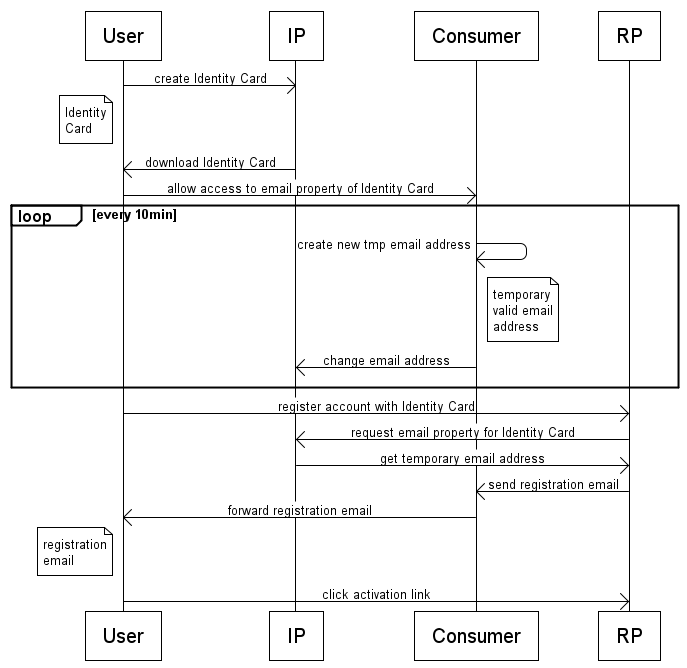
\includegraphics[width=\textwidth]{../HPI-IP-OAuth/raw/master/example-service-seq.png}
	\caption{Sequence diagram of the proposed privacy service.}  
\end{figure}


\subsection{Implementation}

Our example service has to be a webservice able to receive and send
emails. Because we were not in control of and did not want to set
up an own SMTP server we choose to use Google AppEngine. \cite{gae}

Google AppEngine is a \emph{Plattform as a Service} infrastructure
framework provided by Google. Developers can use Python and Java
(in fact every programming language that can be run on the Java VM)
to programm web applications for this infrastructure. Like most web
frameworks Google AppEngine also implements the
\emph{Model-View-Controller (MVC) pattern}. The framework also has
APIs to receive and send emails and start Cron jobs. \cite{gae-mail} \cite{gae-cron}   

When an user clicks on the ``Login with HPI IP'' button on the service
application website he will be redirected to the HPI IP where he
can login and grant access to the service. After granting access he
then will be redirected back to the application and can complete
the setup. The service is now able to access the restricted
ressources in behalf of the user.

We can configure a cron job that will call a specific method
recurrently every 10 minutes to set up a new temporary email
address and use the API of the HPI IP to store it as configured by
the user. The same email address is stored by the service and
associated with the real email address of the user.

Applications running on Google AppEngine are able to receive and
send mails. When the service receives an email it looks for the
this address in the temporary email address table. If it exists the
email will be redirected to the associated actual email address of
the user. Otherwise the email will be ignored.
